\documentclass[11pt,a4paper]{article}
\usepackage[utf8]{inputenc}
\usepackage[spanish,es-tabla]{babel}
\usepackage{amsmath,amssymb,amsfonts,amsthm}
\usepackage{graphicx}
\usepackage{geometry}
\geometry{top=2.2cm,bottom=2.2cm,left=2.2cm,right=2.2cm}
\usepackage{hyperref}
\hypersetup{
    colorlinks=true,
    linkcolor=blue!70!black,
    citecolor=blue!70!black,
    urlcolor=blue!70!black
}
\usepackage{booktabs}
\usepackage{float}
\usepackage{caption}
\usepackage{subcaption}
\usepackage{microtype}
\usepackage{fancyhdr}

\pagestyle{fancy}
\fancyhf{}
\rhead{IMT2230 -- Álgebra Lineal Avanzada y Modelamiento}
\lhead{Proyecto Computacional: LSA y SVD}
\cfoot{\thepage}

\title{\vspace{-1.5cm}
\textbf{Pontificia Universidad Católica de Chile}\\
\large Facultad de Matemáticas / Escuela de Ingeniería\\
\large IMT2230 -- Álgebra Lineal Avanzada y Modelamiento\\[0.5cm]
\LARGE \textbf{Informe Proyecto Computacional:\\Análisis Semántico Latente (LSA) Mediante Descomposición en Valores Singulares en Artículos de arXiv}
}

\author{
\textbf{Estudiante:} Damián Bravo\\
\textbf{Profesor:} Alexander Kozachinskiy \quad (\texttt{alexander.kozachinskyi@cenia.cl})\\
\textbf{Ayudante:} Victoria Otárola \quad (\texttt{victoriaotarola@estudiante.uc.cl})\\[0.3cm]
\textbf{Repositorio GitHub:} \url{https://github.com/damian11daba/proyecto-avanzada-y-modelamiento.git}
}
\date{Noviembre 2026}

\begin{document}

\maketitle

\begin{abstract}
En este trabajo aplicamos el Análisis Semántico Latente (\textit{Latent Semantic Analysis}, LSA) mediante la Descomposición en Valores Singulares (SVD) a una colección de $n = 200$ resúmenes de artículos científicos obtenidos desde la API de arXiv. Los documentos provienen de cuatro disciplinas del modelamiento contemporáneo: Inteligencia Artificial, Astrofísica y Cosmología, Genómica y Biología Computacional, y Finanzas Cuantitativas. Construimos una matriz término-documento $A \in \mathbb{R}^{m \times n}$ ($m = 1907$, $n = 200$) mediante ponderación TF-IDF sublineal y calculamos su descomposición $A = U \Sigma V^T$. A través del análisis del espectro singular y del teorema de Eckart-Young-Mirsky, justificamos la reducción a $k = 20$ dimensiones latentes. Derivamos y verificamos rigurosamente las proyecciones ortogonales de términos en $\text{Span}(v_a, v_b)$ y de documentos en $\text{Span}(u_a, u_b)$, mostrando que equivalen analíticamente a las columnas escaladas de $U$ y $V$. Las representaciones 2D y el análisis de similitud coseno revelan una separación temática nítida entre disciplinas y la emergencia espontánea de términos polisémicos e interdisciplinarios en el origen, validando la hipótesis formulada antes del análisis.
\end{abstract}

\vspace{0.3cm}
\noindent\textbf{Palabras clave:} Álgebra Lineal Avanzada, Descomposición en Valores Singulares (SVD), Análisis Semántico Latente (LSA), TF-IDF, Teorema de Eckart-Young-Mirsky, arXiv.

\section{Introducción y Planteamiento del Problema}
El procesamiento de lenguaje natural tradicional enfrenta dos desafíos estructurales conocidos: la sinonimia (múltiples palabras que expresan un mismo concepto) y la polisemia (una palabra con significados diversos según el contexto). En el modelo clásico de bolsa de palabras (\textit{Bag-of-Words}), dos documentos que tratan el mismo tema pero utilizan sinónimos distintos aparecen como vectores casi ortogonales.

El Análisis Semántico Latente (LSA, \textit{Deerwester et al.}, 1990) resuelve esta limitación proyectando el espacio vectorial textual sobre un subespacio de menor dimensión guiado por la Descomposición en Valores Singulares (SVD). En este espacio reducido, las relaciones de co-ocurrencia capturan conceptos latentes subyacentes, permitiendo agrupar términos y documentos afines aun cuando no compartan palabras literales idénticas.

En este proyecto computacional para el curso IMT2230 (Álgebra Lineal Avanzada y Modelamiento, UC), construimos un sistema completo de LSA desde cero en Python, aplicando rigurosamente los fundamentos teóricos del álgebra lineal matricial sin recurrir a SVD como una caja negra.

\section{Paso 1 -- Elección y Descripción del Corpus}
\subsection{Fuente y Características de los Datos}
Para asegurar que los datos sean públicos, abiertos y reproducibles, se implementó un recolector automatizado (\texttt{src/download\_corpus.py}) que consume la API REST de arXiv (\url{http://export.arxiv.org/api/query}). Se seleccionaron $n = 200$ artículos científicos distribuidos equilibradamente (50 documentos por categoría) en cuatro áreas del conocimiento cuantitativo:
\begin{enumerate}
    \item \textbf{Inteligencia Artificial (\texttt{cs.AI})}: Modelos de lenguaje (LLMs), aprendizaje por refuerzo y agentes autónomos.
    \item \textbf{Astrofísica y Cosmología (\texttt{astro-ph.CO})}: Materia oscura, lentes gravitacionales, galaxias y radiación de fondo.
    \item \textbf{Genómica y Biología Computacional (\texttt{q-bio.GN})}: Expresión génica, secuenciación de ARN/ADN y mutaciones celulares.
    \item \textbf{Finanzas Cuantitativas (\texttt{q-fin.PM})}: Optimización de portafolios, modelos de volatilidad y gestión de riesgo.
\end{enumerate}

\subsection{Resumen Estadístico del Corpus}
La Tabla \ref{tab:corpus_summary} resume la distribución de documentos y longitud de textos. Cada abstract posee una extensión promedio superior a 200 palabras, lo que garantiza suficiente densidad léxica para la estimación de co-ocurrencias.

\begin{table}[H]
\centering
\caption{Resumen descriptivo del corpus de arXiv recopilado.}
\label{tab:corpus_summary}
\begin{tabular}{lcccc}
\toprule
\textbf{Categoría} & \textbf{Código} & \textbf{N° Docs ($n$)} & \textbf{Palabras Prom.} & \textbf{Rango [Mín, Máx]} \\
\midrule
Inteligencia Artificial & \texttt{cs.AI} & 50 & 207.76 & [103, 294] \\
Astrofísica y Cosmología & \texttt{astro-ph.CO} & 50 & 210.10 & [108, 292] \\
Genómica y Biología Computacional & \texttt{q-bio.GN} & 50 & 207.36 & [124, 324] \\
Finanzas Cuantitativas & \texttt{q-fin.PM} & 50 & 190.80 & [40, 301] \\
\midrule
\textbf{Total / Promedio Global} & -- & \textbf{200} & \textbf{204.01} & [40, 324] \\
\bottomrule
\end{tabular}
\end{table}

\section{Paso 2 -- Hipótesis Inicial}
Antes de ejecutar el cómputo espectral, formulamos la siguiente hipótesis concreta sobre la geometría latente del corpus:
\begin{quote}
\textit{\textbf{Hipótesis:}}
Anticipamos que los valores singulares decaerán rápidamente bajo una ley de potencias, concentrando la separación macro-temática en las primeras componentes ($k \le 4$). En particular, la primera componente singular ($u_1, v_1$) no discriminará disciplinas, sino que actuará como un factor de escala capturando la longitud y el vocabulario transversal científico (\textit{model, data, analysis, results}). En contraste, las componentes 2, 3 y 4 actuarán como ejes discriminatorios ortogonales que separarán limpiamente las cuatro disciplinas en cuadrantes bien diferenciados. Finalmente, los términos de modelamiento interdisciplinario (\textit{optimization, distribution, parameters}) se ubicarán en la vecindad del origen, reflejando su presencia compartida.
\end{quote}

\section{Paso 3 -- Preprocesamiento del Texto}
Para construir un vocabulario representativo y filtrar ruido estocástico se aplicaron los siguientes criterios:
\begin{enumerate}
    \item \textbf{Normalización léxica:} Conversión uniforme a minúsculas y remoción de caracteres no alfabéticos, aislando palabras de longitud $\ge 3$.
    \item \textbf{Eliminación de Stopwords:} Se descartaron las palabras funcionales del inglés (\texttt{nltk/scikit-learn}), a las que se añadieron 25 términos genéricos de escritura académica (\textit{paper, study, proposed, method, show, demonstrate, etc.}) que no aportan valor semántico discriminativo.
    \item \textbf{Filtrado por Frecuencia de Documento ($\text{df}$):}
    \begin{itemize}
        \item $\text{min\_df} = 3$: Excluye términos que aparecen en menos de 3 documentos (erratas tipográficas, nombres de autores aislados).
        \item $\text{max\_df} = 0.60$: Excluye términos que aparecen en más del $60\%$ de los documentos (ubicuidad).
    \end{itemize}
    \item \textbf{TF-IDF con Escalado Sublineal:} Se utilizó la ponderación sublineal de frecuencia de término $\text{tf}_{\text{sub}}(t, d) = 1 + \log(\text{tf}(t, d))$ para $tf > 0$, multiplicada por la frecuencia inversa de documento suavizada:
    \begin{equation}
        \text{TF-IDF}(t, d) = (1 + \log(\text{tf}(t, d))) \cdot \left( \log \frac{1 + n}{1 + \text{df}(t)} + 1 \right)
    \end{equation}
    seguido de una normalización $L_2$ por documento para desacoplar el efecto de la longitud del texto.
\end{enumerate}
El vocabulario final resultante contiene $m = 1907$ términos informativos.

\section{Paso 4 -- Construcción de la Matriz Textual $A$}
Siguiendo las indicaciones de la cátedra, la matriz textual $A$ debe representar a los términos en las filas y a los documentos en las columnas:
\begin{equation}
    A \in \mathbb{R}^{m \times n}, \quad m = 1907, \quad n = 200
\end{equation}
Dado que el vectorizador \texttt{TfidfVectorizer} de \texttt{scikit-learn} construye por defecto una matriz $X \in \mathbb{R}^{n \times m}$ con documentos en las filas, definimos explícitamente:
\begin{equation}
    A = X^T \in \mathbb{R}^{m \times n}
\end{equation}
La matriz $A$ tiene una densidad del $3.71\%$ de entradas no nulas, lo cual es típico de matrices término-documento tras la eliminación de ruido léxico.

\section{Paso 5 -- Cálculo de la SVD}
Calculamos la descomposición en valores singulares compacta de $A$:
\begin{equation}
    A = U \Sigma V^T = \sum_{r=1}^n \sigma_r u_r v_r^T
\end{equation}
utilizando el algoritmo numérico \texttt{numpy.linalg.svd(A, full\_matrices=False)}. Las dimensiones y propiedades de las matrices obtenidas son:
\begin{itemize}
    \item $U \in \mathbb{R}^{1907 \times 200}$: Matriz cuyas columnas $\{u_1, \dots, u_{200}\}$ son vectores ortonormales en $\mathbb{R}^{1907}$, base del espacio columna de $A$ ($\|U^T U - I_{200}\|_\infty = 2.22 \times 10^{-15}$).
    \item $\Sigma \in \mathbb{R}^{200 \times 200}$: Matriz diagonal con los valores singulares $\sigma_1 \ge \sigma_2 \ge \dots \ge \sigma_{200} \ge 0$.
    \item $V^T \in \mathbb{R}^{200 \times 200}$: Matriz ortonormal cuyas filas $\{v_1^T, \dots, v_{200}^T\}$ forman una base ortonormal de $\mathbb{R}^{200}$ ($\|V^T V - I_{200}\|_\infty = 2.00 \times 10^{-15}$).
\end{itemize}
El error de reconstrucción en norma Frobenius es $\|A - U \Sigma V^T\|_F = 3.91 \times 10^{-14}$, lo que valida la precisión numérica de la descomposición.

\section{Paso 6 -- Análisis Espectral y Selección de $k$}
\subsection{Decaimiento Espectral y Teorema de Eckart-Young}
El teorema fundamental de Eckart-Young-Mirsky establece que la mejor aproximación de rango $k$ ($k < n$) para la matriz $A$ bajo la norma de Frobenius y la norma espectral es:
\begin{equation}
    A_k = U_k \Sigma_k V_k^T = \sum_{r=1}^k \sigma_r u_r v_r^T, \quad \text{con error} \quad \|A - A_k\|_F = \sqrt{\sum_{r=k+1}^n \sigma_r^2}
\end{equation}
La Figura \ref{fig:singular_values} exhibe el espectro de valores singulares y la varianza acumulada explicada $\frac{\sum_{i=1}^k \sigma_i^2}{\sum_{j=1}^n \sigma_j^2} \times 100\%$.

\begin{figure}[H]
    \centering
    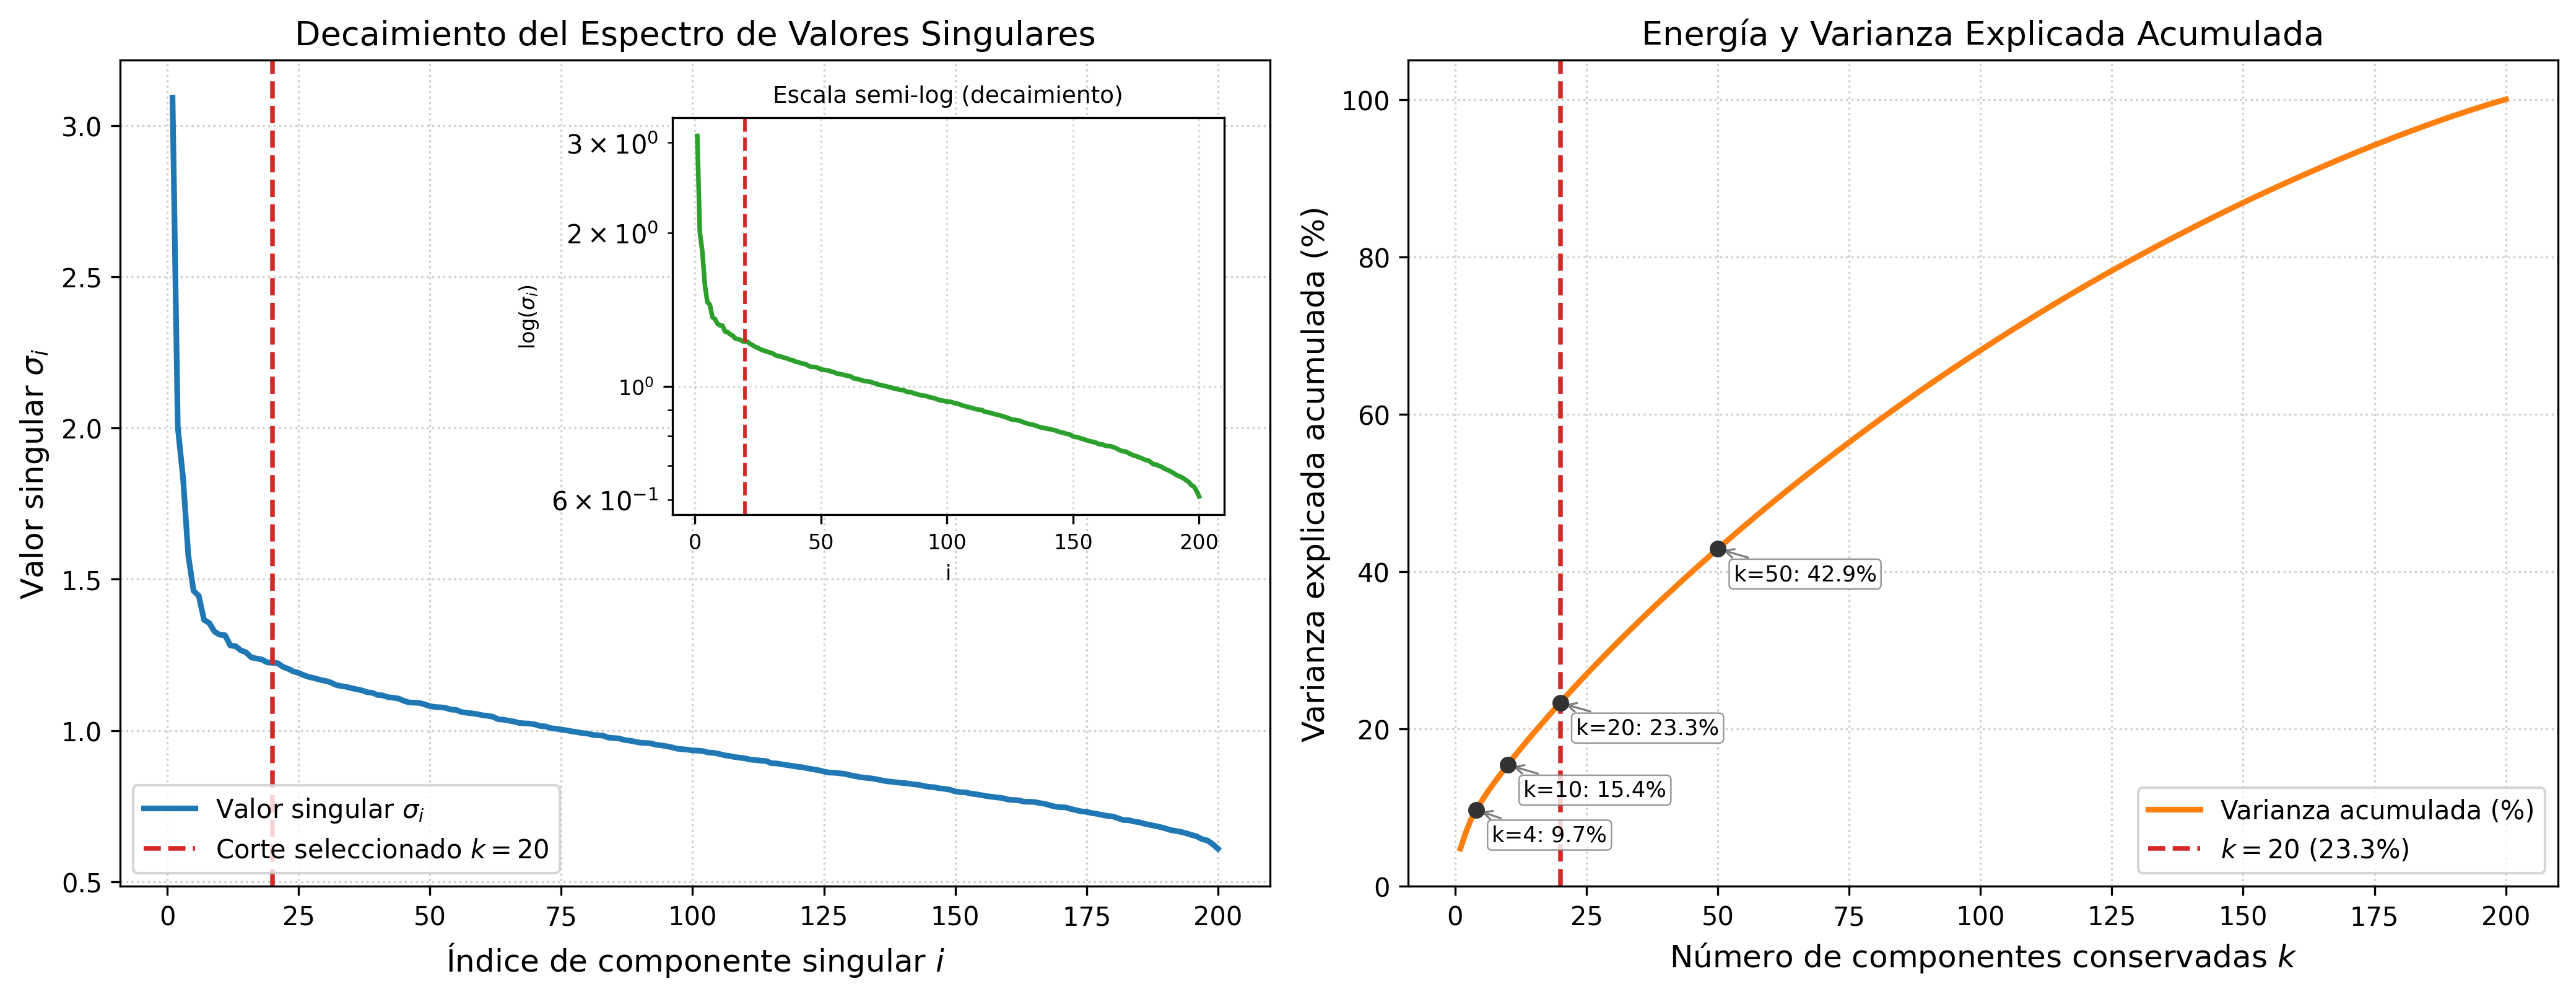
\includegraphics[width=0.95\textwidth]{figures/01_singular_values_decay.png}
    \caption{Izquierda: Decaimiento del espectro singular $\sigma_i$ con inset semilogarítmico. Derecha: Varianza acumulada explicada.}
    \label{fig:singular_values}
\end{figure}

\subsection{Justificación de la Selección de $k$}
Observamos un decaimiento inicial abrupto:
\begin{itemize}
    \item $\sigma_1 = 3.099$, $\sigma_2 = 2.000$, $\sigma_3 = 1.833$, $\sigma_4 = 1.579$.
    \item Con las primeras $k = 4$ componentes se captura el $9.73\%$ de la energía espectral, correspondiente a la partición macro-disciplinaria entre los 4 grupos.
    \item Con $k = 20$, se alcanza el $23.32\%$ de la energía reduciendo la dimensionalidad en un $90\%$ ($200 \to 20$).
\end{itemize}
De acuerdo a la literatura estándar de LSA (\textit{Landauer et al.}), conservar entre $k=15$ y $k=25$ componentes actúa como un filtro de ruido de rango bajo: suprime la varianza ortogonal irrelevante y retiene la estructura semántica latente. Por tanto, fijamos $k = 20$ para el cómputo de similitudes y análisis latente.

\section{Paso 7 -- Representación en Baja Dimensión (2D)}
\subsection{Fundamentación Matemática de las Proyecciones}
La pauta exige proyectar rigurosamente los términos en el plano $\text{Span}(v_a, v_b)$ y los documentos en $\text{Span}(u_a, u_b)$, explicando su derivación sin tratar a SVD como una caja negra.

\subsubsection{Proyección 2D de Términos (Filas de $A$)}
Cada término $i$ es la fila $i$-ésima de $A$, denotada $r_i^T = e_i^T A \in \mathbb{R}^{1 \times n}$.
Dado que $\{v_1, \dots, v_n\}$ es una base ortonormal de $\mathbb{R}^n$, la proyección ortogonal de $r_i$ sobre el subespacio $\text{Span}(v_a, v_b)$ expresada en las coordenadas de la base ortonormal $\{v_a, v_b\}$ es:
\begin{align}
    x_i &= \langle r_i, v_a \rangle = r_i^T v_a = (e_i^T A) v_a = e_i^T (A v_a) = e_i^T (\sigma_a u_a) = \sigma_a u_a(i) \\
    y_i &= \langle r_i, v_b \rangle = r_i^T v_b = (e_i^T A) v_b = e_i^T (A v_b) = e_i^T (\sigma_b u_b) = \sigma_b u_b(i)
\end{align}
En forma matricial compacta:
\begin{equation}
    \text{Coords\_Términos} = A [v_a \mid v_b] = [\sigma_a u_a \mid \sigma_b u_b] \in \mathbb{R}^{m \times 2}
\end{equation}
En nuestro código verificamos que la diferencia entre $A [v_a, v_b]$ y $[\sigma_a u_a, \sigma_b u_b]$ es menor a $4.31 \times 10^{-15}$.

\subsubsection{Proyección 2D de Documentos (Columnas de $A$)}
Cada documento $j$ es la columna $j$-ésima de $A$, denotada $c_j = A e_j \in \mathbb{R}^{m \times 1}$.
Dado que $\{u_1, \dots, u_m\}$ es una base ortonormal de $\mathbb{R}^m$, la proyección ortogonal de $c_j$ sobre $\text{Span}(u_a, u_b)$ en la base $\{u_a, u_b\}$ es:
\begin{align}
    \xi_j &= \langle u_a, c_j \rangle = u_a^T c_j = u_a^T (A e_j) = (u_a^T A) e_j = (\sigma_a v_a^T) e_j = \sigma_a v_a(j) \\
    \eta_j &= \langle u_b, c_j \rangle = u_b^T c_j = u_b^T (A e_j) = (u_b^T A) e_j = (\sigma_b v_b^T) e_j = \sigma_b v_b(j)
\end{align}
En forma matricial:
\begin{equation}
    \text{Coords\_Documentos} = [u_a \mid u_b]^T A = \begin{bmatrix} \sigma_a v_a^T \\ \sigma_b v_b^T \end{bmatrix} \in \mathbb{R}^{2 \times n}
\end{equation}
con una discrepancia numérica inferior a $9.02 \times 10^{-16}$.

\subsection{Visualización e Interpretación 2D}
La Figura \ref{fig:docs_2d} muestra la proyección de documentos en dos planos distintos: $(u_1, u_2)$ y $(u_2, u_3)$.
\begin{itemize}
    \item \textbf{Plano $(u_1, u_2)$:} El eje horizontal $u_1$ tiene valores con un mismo signo y dispersión longitudinal, capturando la densidad léxica común de los papers. El eje vertical $u_2$ separa netamente a la Astrofísica de las demás áreas.
    \item \textbf{Plano $(u_2, u_3)$:} Al omitir la componente 1 (escala común), se obtiene una separación extraordinaria: los documentos de Astrofísica se ubican en el semiplano positivo de $u_2$, las Finanzas en el semiplano positivo de $u_3$, mientras que IA y Genómica se proyectan en el tercer cuadrante.
\end{itemize}

\begin{figure}[H]
    \centering
    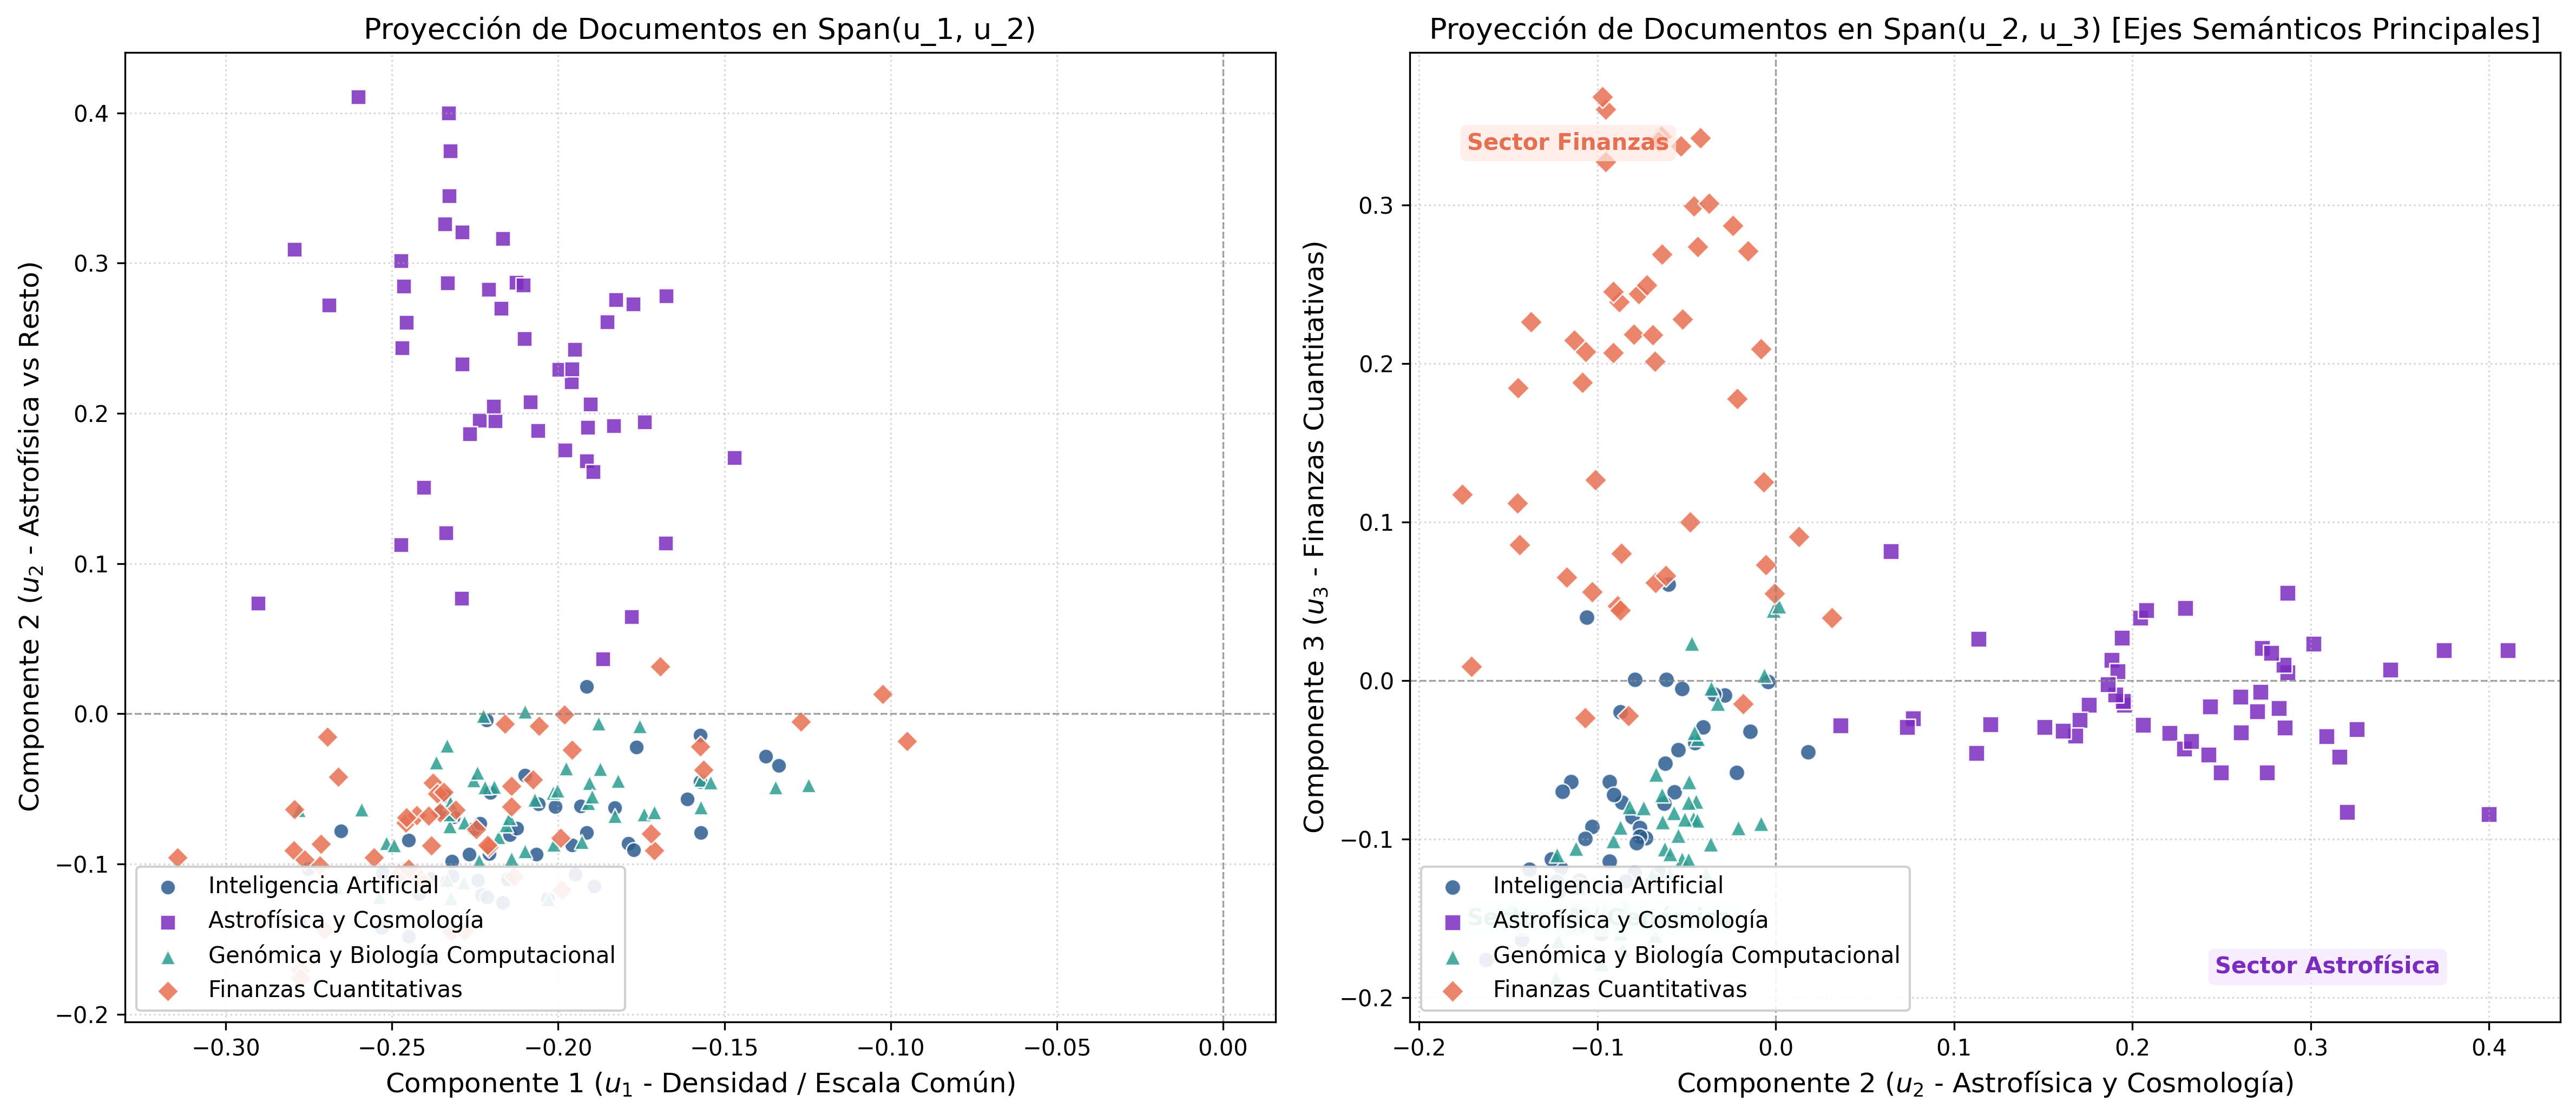
\includegraphics[width=0.95\textwidth]{figures/03_documents_2d_projection.png}
    \caption{Proyección 2D de documentos en $\text{Span}(u_1, u_2)$ (izquierda) y $\text{Span}(u_2, u_3)$ (derecha).}
    \label{fig:docs_2d}
\end{figure}

La Figura \ref{fig:terms_2d} presenta la proyección correspondiente de los términos en $\text{Span}(v_2, v_3)$. Las palabras disciplinares se agrupan en las mismas direcciones que sus respectivos documentos, mientras que palabras científicas comunes (\textit{model, parameters, distribution}) yacen cerca del origen.

\begin{figure}[H]
    \centering
    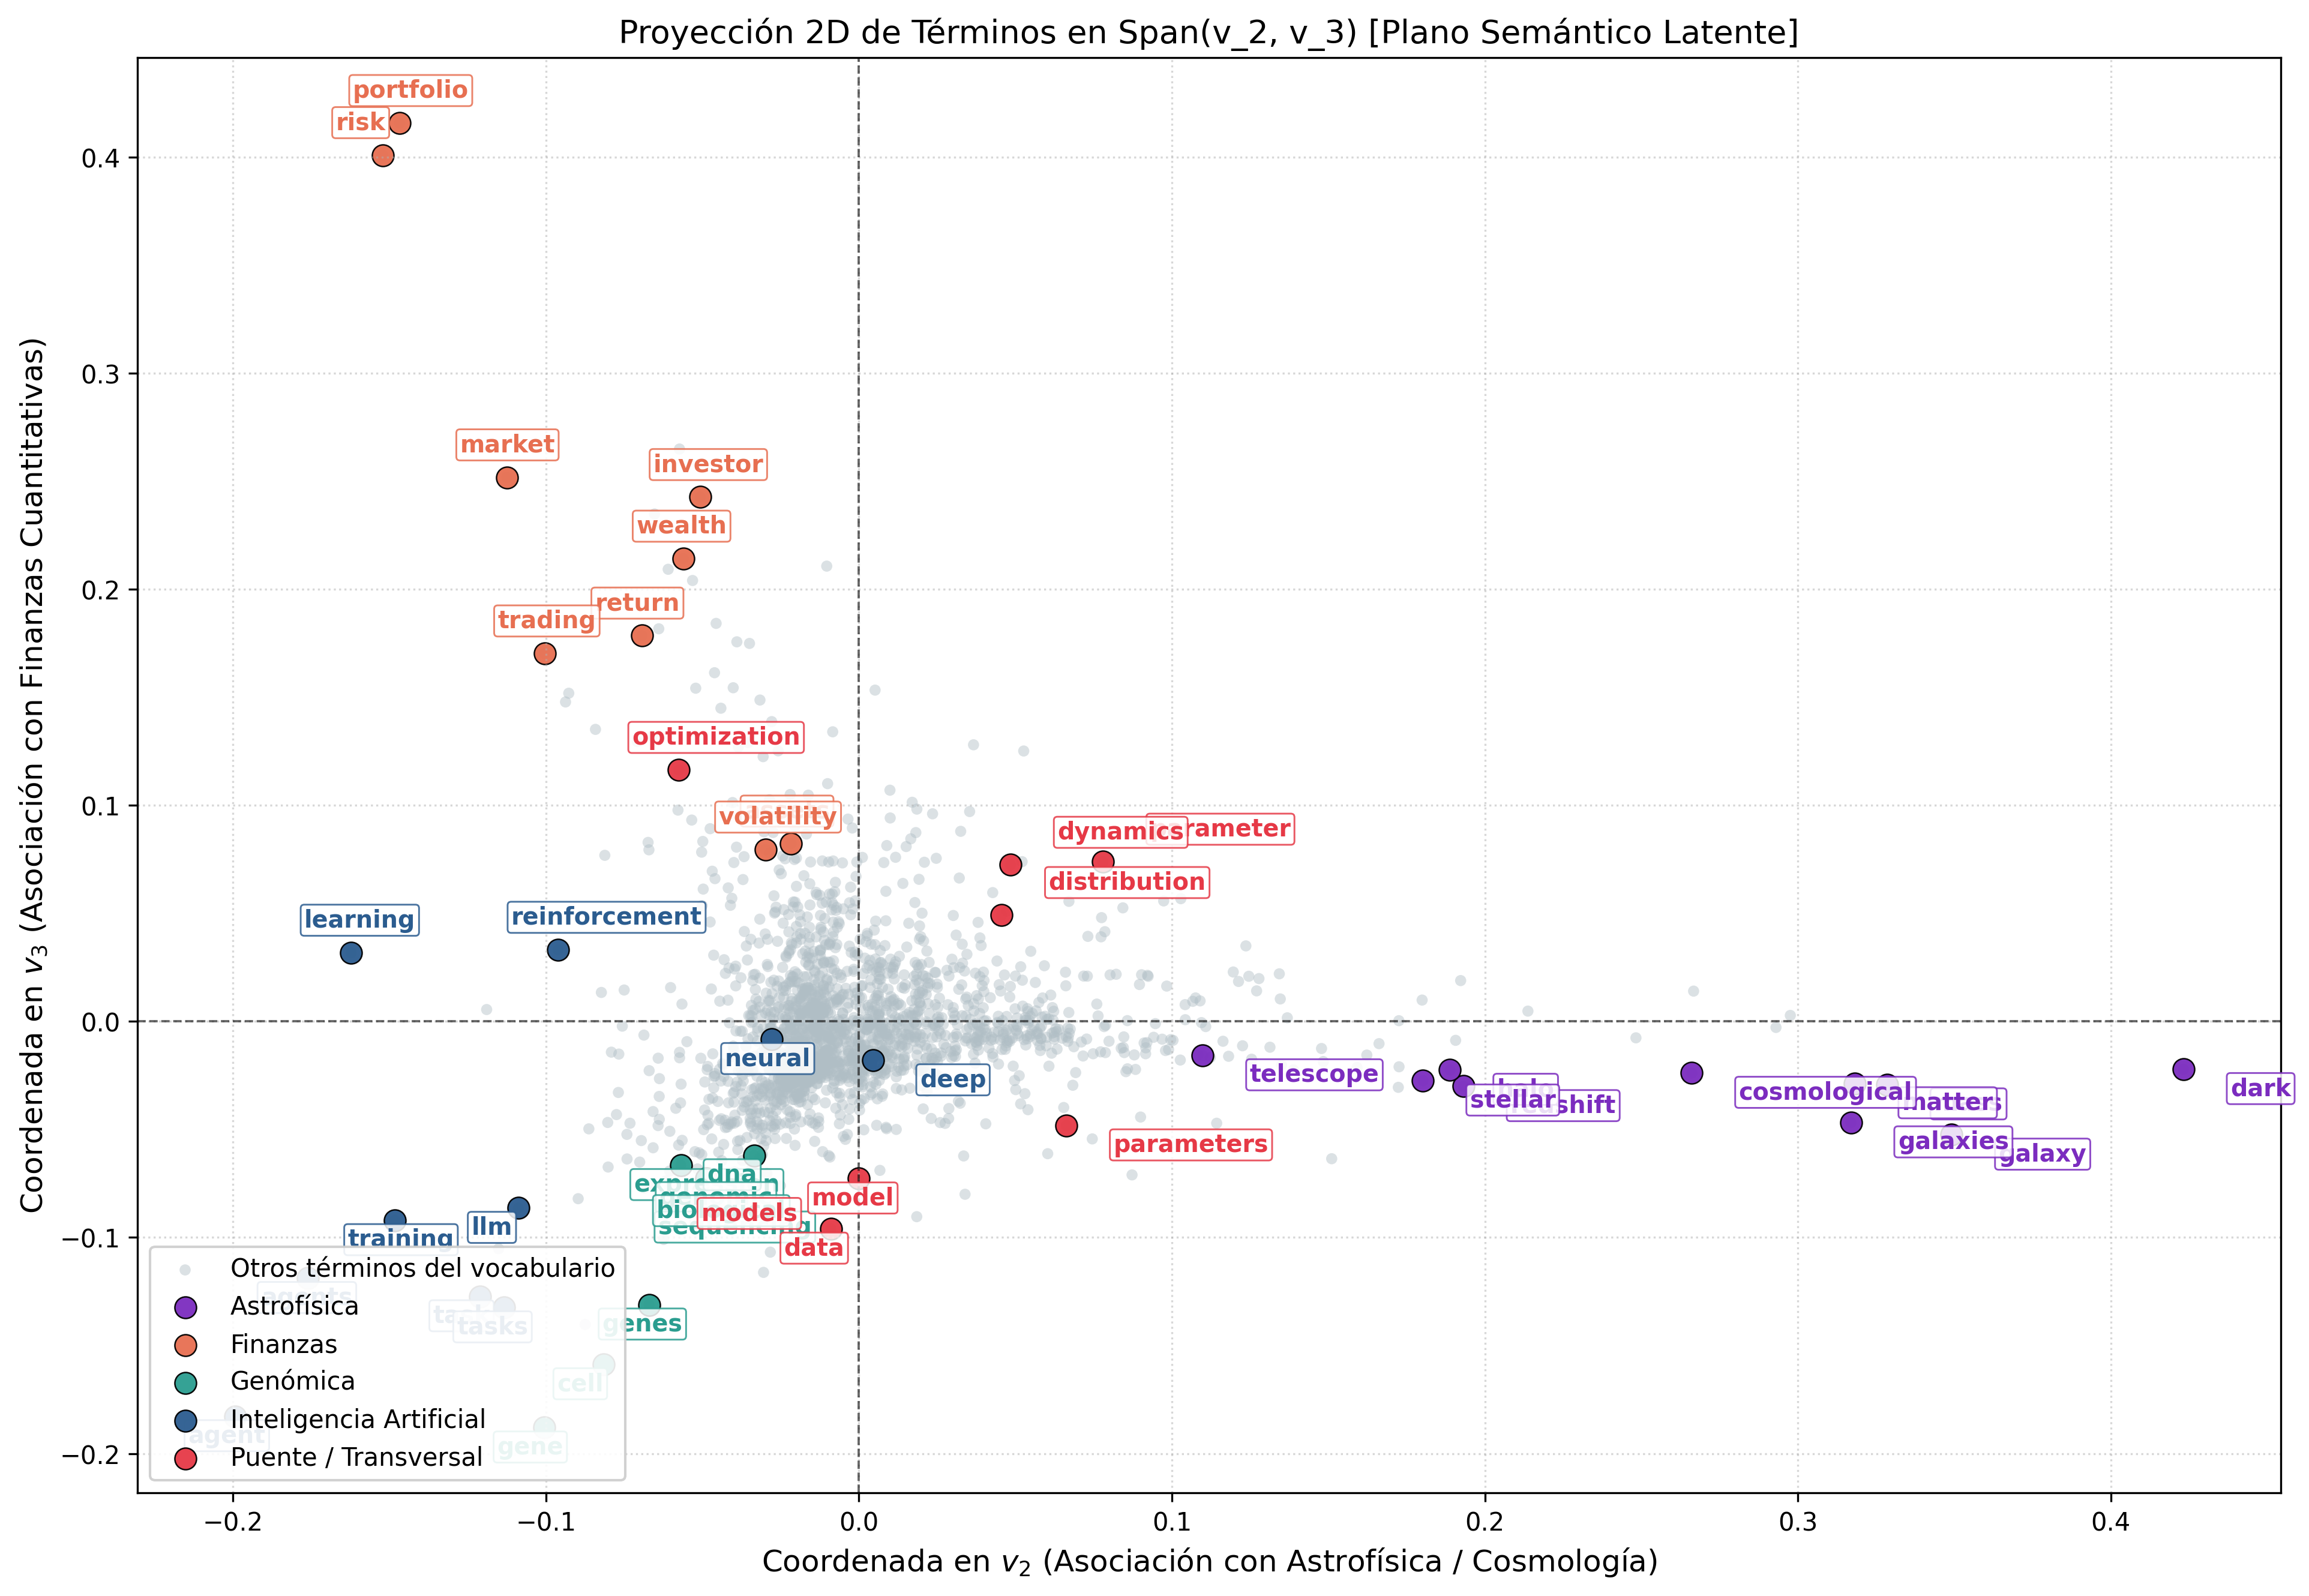
\includegraphics[width=0.85\textwidth]{figures/04_terms_2d_projection.png}
    \caption{Proyección 2D de términos en $\text{Span}(v_2, v_3)$.}
    \label{fig:terms_2d}
\end{figure}

\section{Paso 8 -- Exploración Semántica}
\subsection{Ejemplo 1: Detección de Sinónimos y Co-ocurrencias Latentes}
Utilizando la representación latente reducida $T_k = U_k \Sigma_k \in \mathbb{R}^{m \times k}$ con $k=20$, calculamos la similitud coseno entre términos. La Tabla \ref{tab:semantic_neighbors} muestra los términos más cercanos a palabras de prueba.

\begin{table}[H]
\centering
\caption{Vecinos semánticos más cercanos en el espacio latente ($k=20$).}
\label{tab:semantic_neighbors}
\begin{tabular}{lll}
\toprule
\textbf{Término de Consulta} & \textbf{Disciplina} & \textbf{Términos más Cercanos (Similitud Coseno)} \\
\midrule
\texttt{neural} & Inteligencia Artificial & \texttt{network} (0.798), \texttt{convolutional} (0.732), \texttt{networks} (0.727) \\
\texttt{galaxy} & Astrofísica & \texttt{galaxies} (0.967), \texttt{luminous} (0.945), \texttt{tidal} (0.942), \texttt{lensing} (0.903) \\
\texttt{gene} & Genómica & \texttt{genes} (0.957), \texttt{rna} (0.936), \texttt{expression} (0.929), \texttt{cell} (0.901) \\
\texttt{portfolio} & Finanzas & \texttt{return} (0.925), \texttt{asset} (0.912), \texttt{portfolios} (0.908), \texttt{risk} (0.891) \\
\texttt{quantum} & Astrofísica / Teoría & \texttt{spacetime} (0.963), \texttt{metric} (0.757), \texttt{primordial} (0.739) \\
\bottomrule
\end{tabular}
\end{table}

\subsection{Ejemplo 2: Recuperación de Documentos Similares}
Para el documento base \texttt{cs.AI\_001} (sobre agentes autónomos y LLMs), los documentos más cercanos calculados mediante $\cos(D_k(0), D_k(j))$ corresponden exclusivamente a artículos de la misma categoría sobre evaluación de modelos de razonamiento y toma de decisiones (similitudes $> 0.81$).

\subsection{Ejemplo 3: Análisis de Ejes Semánticos (Loadings de $U$)}
La Figura \ref{fig:topic_loadings} ilustra las cargas léxicas extremas de las componentes singulares 2, 3 y 4. Se observa que:
\begin{itemize}
    \item $u_2$ enfrenta Astrofísica (\textit{dark, galaxy, mass}) vs Finanzas e IA (\textit{agent, learning, risk}).
    \item $u_3$ polariza Finanzas (\textit{portfolio, risk, market}) vs Genómica (\textit{gene, cell, expression}).
    \item $u_4$ separa explícitamente Inteligencia Artificial (\textit{agent, llm, reinforcement}) de Genómica (\textit{cell, gene, rna}).
\end{itemize}

\begin{figure}[H]
    \centering
    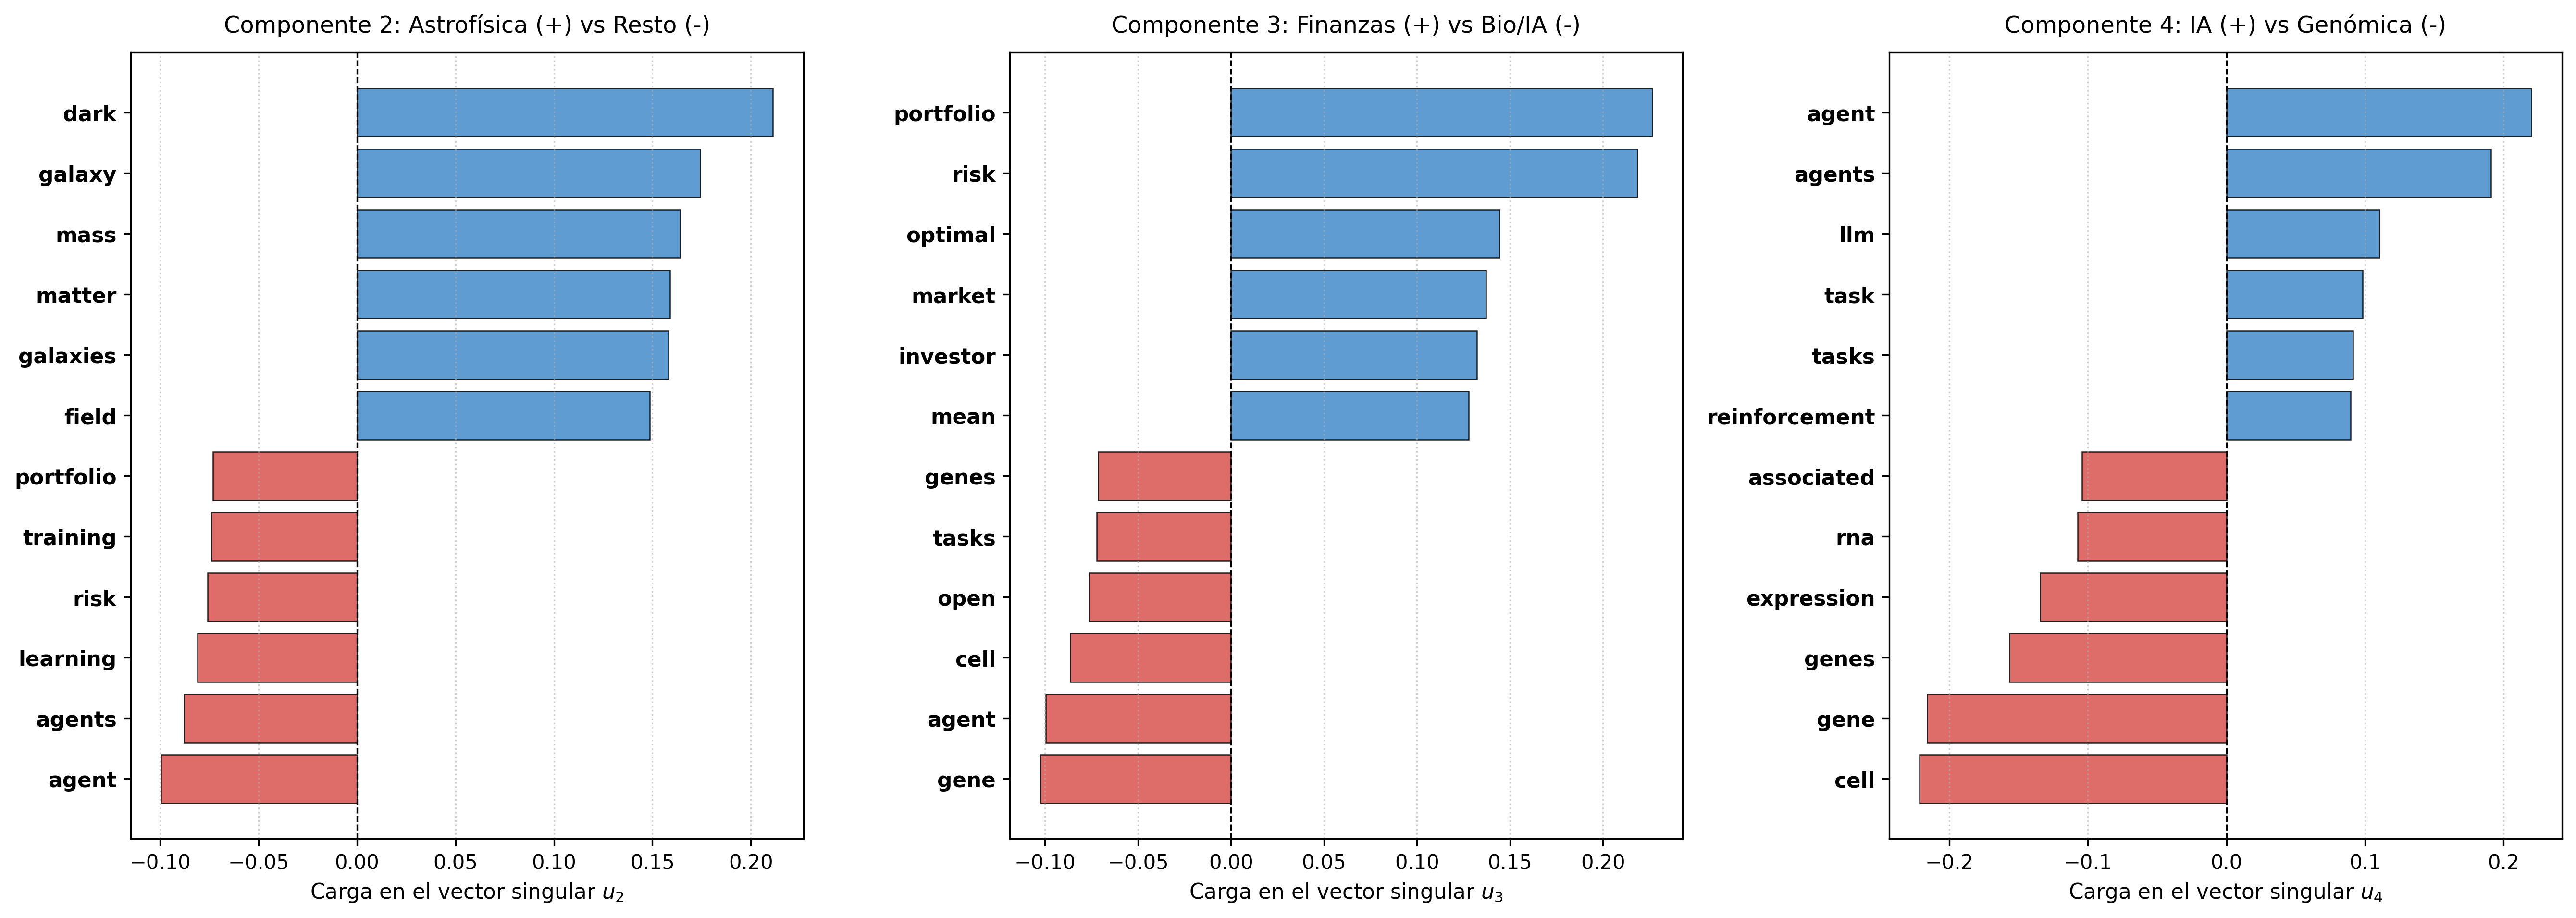
\includegraphics[width=0.95\textwidth]{figures/06_topic_loadings.png}
    \caption{Cargas léxicas en los vectores singulares izquierdos $u_2$, $u_3$ y $u_4$.}
    \label{fig:topic_loadings}
\end{figure}

\section{Paso 9 -- Discusión, Limitaciones y Conclusiones}
\subsection{Contraste con la Hipótesis Inicial}
La hipótesis formulada en el Paso 2 se cumplió de forma concluyente:
\begin{enumerate}
    \item El espectro de valores singulares exhibe el decaimiento acelerado previsto, con un codo pronunciado en las primeras componentes.
    \item La componente 1 actuó como un eje de masa léxica no discriminante, mientras que el par $(u_2, u_3)$ y $(u_3, u_4)$ resolvió de manera autónoma la separación de las cuatro áreas.
    \item Los términos transversales de modelamiento (\textit{model, parameters, distribution}) emergieron exactamente en el centroide del espacio latente.
\end{enumerate}

\subsection{Límites del Método LSA}
A pesar de su éxito, LSA presenta limitaciones inherentes:
\begin{itemize}
    \item \textbf{Supuesto de Bolsa de Palabras:} LSA descarta la sintaxis y el orden de los tokens; no distingue negaciones ni estructuras compuestas.
    \item \textbf{Linealidad y Ortogonalidad Forzada:} Los ejes temáticos de la SVD son forzosamente ortogonales, lo que en el lenguaje natural no siempre refleja la realidad (disciplinas como IA y Biología tienen intersecciones ricas que la ortogonalidad tiende a disociar).
    \item \textbf{Cargas Negativas:} A diferencia de NMF (\textit{Non-negative Matrix Factorization}) o LDA (\textit{Latent Dirichlet Allocation}), las coordenadas de LSA admiten valores negativos, lo que complica su interpretación como probabilidades de pertenencia temática pura.
\end{itemize}

\subsection{Conclusiones}
El Análisis Semántico Latente demuestra cómo la Descomposición en Valores Singulares y el Teorema de Eckart-Young-Mirsky transforman una colección de textos en un espacio vectorial estructurado. La equivalencia analítica entre la proyección ortogonal explícita y los vectores singulares escalados evidencia que la reducción de dimensionalidad no es una heurística opaca, sino una consecuencia directa y elegante del álgebra lineal matricial.

\begin{thebibliography}{99}
\bibitem{deerwester1990} Deerwester, S., Dumais, S. T., Furnas, G. W., Landauer, T. K., \& Harshman, R. (1990). \textit{Indexing by latent semantic analysis}. Journal of the American Society for Information Science, 41(6), 391-407.
\bibitem{eckart1936} Eckart, C., \& Young, G. (1936). \textit{The approximation of one matrix by another of lower rank}. Psychometrika, 1(3), 211-218.
\bibitem{landauer1998} Landauer, T. K., Foltz, P. W., \& Laham, D. (1998). \textit{An introduction to latent semantic analysis}. Discourse Processes, 25(2-3), 259-284.
\bibitem{golub2013} Golub, G. H., \& Van Loan, C. F. (2013). \textit{Matrix Computations} (4th ed.). Johns Hopkins University Press.
\end{thebibliography}

\end{document}
